\documentclass[tikz,border=10pt]{standalone}
% No extra TikZ libraries needed.
\begin{document}
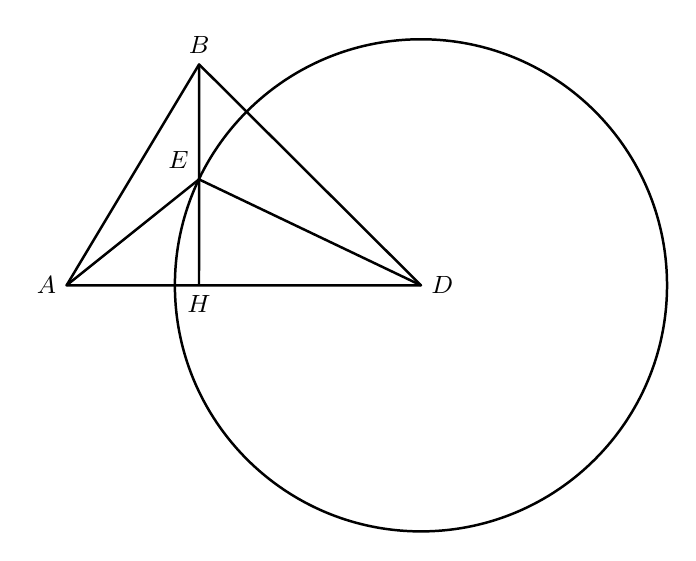
\begin{tikzpicture}[line width=0.9pt, line join=round,
  lbl/.style={font=\fontsize{9.5}{11.4}\selectfont}]
  % Named points (scale s = 0.01194 units/px, origin shifted to image ink centre)
  \coordinate (A) at (-3.652,0);
  \coordinate (D) at (0.849,0);
  \coordinate (B) at (-1.969,2.806);
  \coordinate (E) at (-1.970,1.346);
  \coordinate (H) at (-1.970,0);

  % Triangle ABD
  \draw (A) -- (B) -- (D) -- cycle;
  % Altitude BH (H on AD)
  \draw (B) -- (H);
  % Segments AE and ED
  \draw (A) -- (E);
  \draw (E) -- (D);

  % Circle centred at D through E (radius |DE| = 3.125)
  \draw (D) circle[radius=3.125];

  % Vertex labels
  \node[lbl, left] at (A) {$A$};
  \node[lbl, above] at (B) {$B$};
  \node[lbl, right] at (D) {$D$};
  \node[lbl, above left] at (E) {$E$};
  \node[lbl, below] at (H) {$H$};
\end{tikzpicture}
\end{document}